% =====================================================================
%  Least squares as orthogonal projection
%  A Chalk rendering test that is also a real piece of mathematics.
%  Mirrors test-docs/least-squares.md section by section, so the two
%  surface syntaxes can be compared box for box.
%
%  COMPILATION: everything up to \section{Edge cases} compiles with
%  pdflatex under the preamble below. The Edge cases section does NOT
%  compile on purpose (undefined environments, unterminated blocks); it
%  exists to exercise the live preview, which must stay well-behaved on
%  input a compiler would reject.
% =====================================================================

\documentclass[11pt]{article}

\usepackage{amsmath, amssymb, amsthm}
\usepackage{graphicx}
\usepackage{booktabs}
\usepackage{hyperref}

\graphicspath{{figures/}}

\newtheorem{theorem}{Theorem}
\newtheorem{lemma}[theorem]{Lemma}
\newtheorem{corollary}[theorem]{Corollary}
\newtheorem{proposition}[theorem]{Proposition}
\newtheorem{conjecture}[theorem]{Conjecture}
\theoremstyle{definition}
\newtheorem{definition}[theorem]{Definition}
\newtheorem{example}[theorem]{Example}
\newtheorem{exercise}[theorem]{Exercise}
\theoremstyle{remark}
\newtheorem*{remark}{Remark}
\newtheorem*{solution}{Solution}
% Chalk renders the Quarto admonition names as callouts on the LaTeX side
% too; define them so the document still compiles.
\newtheorem*{note}{Note}
\newtheorem*{tip}{Tip}
\newtheorem*{warning}{Warning}
\newtheorem*{important}{Important}
\newtheorem*{caution}{Caution}

\title{Least squares as orthogonal projection}
\author{Chalk test suite}
\date{2026-08-03}

\begin{document}

\maketitle

Everything below is one connected argument: least squares is nothing but
orthogonal projection onto a column space, and every classical result about it
falls out of that single geometric fact. The final section is a deliberate
stress test and is \emph{not} meant to read as mathematics.

% --------------------------------------------------------------
\section{Setup and notation}
\label{sec:setup}

We observe $n$ pairs $(x_i, y_i)$ and stack them into a vector
$y \in \mathbb{R}^n$ and [cursor]a matrix $X \in \mathbb{R}^{n \times k}$ whose columns are the regressors. Throughout, $k < n$ and $X$ has \textbf{full column rank}, so $X^\top X$ is invertible. The model is
\begin{equation}
    y = X\beta + \varepsilon, \qquad \mathbb{E}[\varepsilon \mid X] = 0,
    \qquad \operatorname{Var}(\varepsilon \mid X) = \sigma^2 I_n .
    \label{eq:model}
\end{equation}
Two objects do all the work, the \emph{hat matrix} and the \emph{residual maker}:
\begin{equation}
    P = X(X^\top X)^{-1} X^\top, \qquad M = I_n - P .
    \label{eq:hat}
\end{equation}
An unnumbered display carries no tag, which is what you want for a throwaway line:
\begin{equation*}
    \|v\|^2 = \langle v, v \rangle = \sum_{i=1}^n v_i^2 .
\end{equation*}
The bracket form does the same:
\[
    \operatorname{tr}(P) = k, \qquad \operatorname{tr}(M) = n - k .
\]
And so does the double-dollar form:
$$
    \hat\sigma^2 = \frac{e^\top e}{n - k} .
$$
Inline math should sit on the text baseline without stretching the line box: the estimator $\hat\beta = (X^\top X)^{-1} X^\top y$, the fitted values $\hat y = Py$, the residuals $e = My$, the paren form \(\operatorname{Var}(\hat\beta) = \sigma^2 (X^\top X)^{-1}\), and a fraction inline, $\frac{e^\top e}{n-k}$, which is taller than the line.

\section{The projection theorem}
\label{sec:projection}

\begin{definition}[Inner product and orthogonality]\label{def:inner}
For $u, v \in \mathbb{R}^n$ write $\langle u, v \rangle = u^\top v$. Vectors
$u$ and $v$ are \textbf{orthogonal}, written $u \perp v$, when
$\langle u, v \rangle = 0$. A vector is orthogonal to a subspace
$S \subseteq \mathbb{R}^n$ when it is orthogonal to every element of $S$, and
the set of all such vectors is the orthogonal complement
\begin{equation}
    S^{\perp} = \{ v \in \mathbb{R}^n : \langle v, s \rangle = 0
                  \text{ for all } s \in S \} .
    \label{eq:complement}
\end{equation}
\end{definition}

\begin{theorem}[Orthogonal projection]\label{thm:projection}
Let $S \subseteq \mathbb{R}^n$ be a subspace and $y \in \mathbb{R}^n$. There is
a unique $\hat y \in S$ minimising $\|y - s\|$ over $s \in S$, and it is the
unique element of $S$ with $y - \hat y \in S^{\perp}$.
\end{theorem}

\begin{proof}
Existence is the usual compactness argument; we prove the characterisation, which is the part we actually use. Suppose $\hat y \in S$ and $y - \hat y \in S^{\perp}$. For any $s \in S$ the difference $\hat y - s$ lies in $S$, so it is orthogonal to $y - \hat y$ and Pythagoras applies:
\begin{equation}
    \|y - s\|^2 = \|(y - \hat y) + (\hat y - s)\|^2
                = \|y - \hat y\|^2 + \|\hat y - s\|^2
                \ge \|y - \hat y\|^2 ,
    \label{eq:pythagoras}
\end{equation}
with equality exactly when $\hat y = s$. That gives both minimality and uniqueness. Conversely, if $\hat y$ minimises the distance, then for every $s \in S$ the scalar function $t \mapsto \|y - \hat y - t s\|^2$ is minimised at $t = 0$; differentiating and setting the derivative to zero gives $\langle y - \hat y, s \rangle = 0$.
\end{proof}

Applying Theorem~\ref{thm:projection} with $S = \operatorname{col}(X)$ turns the
geometry into linear algebra.

\begin{corollary}[Normal equations]\label{cor:normal}
The minimiser of $\|y - X b\|$ over $b \in \mathbb{R}^k$ solves
\begin{equation}
    X^\top X b = X^\top y ,
    \label{eq:normal}
\end{equation}
and under full column rank it is unique,
$\hat\beta = (X^\top X)^{-1} X^\top y$, so $\hat y = Py$ with $P$ as in
\eqref{eq:hat}.
\end{corollary}

\begin{proof}
By Theorem~\ref{thm:projection} the residual $y - Xb$ must be orthogonal to every column of $X$, that is $X^\top (y - Xb) = 0$, which rearranges to \eqref{eq:normal}. Invertibility of $X^\top X$ follows from full column rank.
\end{proof}

\begin{figure}[t]
    \centering
    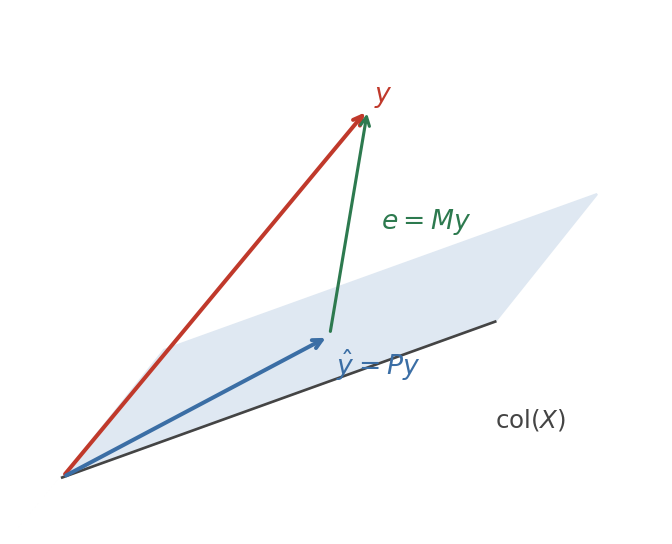
\includegraphics[width=0.55\textwidth]{projection.png}
\caption{Geometry of the projection: $y$ decomposes into $\hat y \in \operatorname{col}(X)$ and $e \perp \operatorname{col}(X)$.}
    \label{fig:projection}
\end{figure}

\section{Consequences}
\label{sec:consequences}

\begin{lemma}[Both projectors are idempotent and symmetric]\label{lem:idem}
$P^\top = P$, $P^2 = P$, $M^\top = M$, $M^2 = M$, and $PM = MP = 0$.
\end{lemma}

\begin{proof}
Symmetry of $P$ is immediate from \eqref{eq:hat} since $(X^\top X)^{-1}$ is
symmetric. For idempotence,
\begin{equation*}
    P^2 = X(X^\top X)^{-1}
          \underbrace{X^\top X (X^\top X)^{-1}}_{= I_k} X^\top = P .
\end{equation*}
The claims about $M = I - P$ follow by expanding, and
$PM = P(I - P) = P - P^2 = 0$.
\end{proof}

\begin{proposition}[Gauss--Markov]\label{prp:gm}
Under \eqref{eq:model}, $\hat\beta$ is unbiased with variance
$\sigma^2 (X^\top X)^{-1}$. Among all linear unbiased estimators
$\tilde\beta = Cy$ it has the smallest variance, in the sense that
$\operatorname{Var}(\tilde\beta) - \operatorname{Var}(\hat\beta)$ is positive
semi-definite.
\end{proposition}

\begin{proof}
Write $C = (X^\top X)^{-1} X^\top + D$. Unbiasedness for every $\beta$ forces
$DX = 0$, and then
\begin{align}
    \operatorname{Var}(\tilde\beta)
      &= \sigma^2 \left[ (X^\top X)^{-1} + D D^\top \right] \nonumber \\
      &= \operatorname{Var}(\hat\beta) + \sigma^2 D D^\top ,
    \label{eq:gm}
\end{align}
because the cross terms carry a factor $DX = 0$. The matrix $DD^\top$ is
positive semi-definite, which is the claim.
\end{proof}

\begin{remark}
Proposition~\ref{prp:gm} is a statement about \emph{linear} estimators only, and it needs homoskedasticity. Drop the second restriction and the efficient estimator is generalised least squares, $\hat\beta_{\mathrm{GLS}} = (X^\top \Omega^{-1} X)^{-1} X^\top \Omega^{-1} y$.
\end{remark}

The decomposition of the sum of squares is now one line. Since $y = Py + My$ with the two pieces orthogonal,
\begin{equation}
    \underbrace{\|y - \bar y \mathbf{1}\|^2}_{\text{TSS}}
      = \underbrace{\|\hat y - \bar y \mathbf{1}\|^2}_{\text{ESS}}
      + \underbrace{\|e\|^2}_{\text{RSS}} ,
    \qquad R^2 = \frac{\text{ESS}}{\text{TSS}}
               = 1 - \frac{\text{RSS}}{\text{TSS}} ,
    \label{eq:anova}
\end{equation}
provided the regression includes an intercept, so that $\mathbf{1} \in \operatorname{col}(X)$.

\begin{warning}
Without an intercept, $\bar e \neq 0$ and \eqref{eq:anova} fails; $R^2$
computed from the usual formula can then be negative. (\texttt{warning} is not a standard amsthm environment, but Chalk recognises the Quarto admonition names on the \LaTeX{} side too.)
\end{warning}

\section{A worked example}
\label{sec:example}

\begin{example}[The bivariate case]\label{exm:bivariate}
With $k = 2$ and $X = [\mathbf{1} \;\; x]$, the normal equations
\eqref{eq:normal} reduce to two scalar equations whose solution is
\begin{align}
    \hat\beta_1 &= \frac{\sum_i (x_i - \bar x)(y_i - \bar y)}
                        {\sum_i (x_i - \bar x)^2}
                 = \frac{\widehat{\operatorname{Cov}}(x, y)}
                        {\widehat{\operatorname{Var}}(x)}, \\
    \hat\beta_0 &= \bar y - \hat\beta_1 \bar x .
    \label{eq:bivariate}
\end{align}
So the slope is a covariance-to-variance ratio and the fitted line passes through the point of means $(\bar x, \bar y)$.
\end{example}

Fitting \eqref{eq:bivariate} to $n = 30$ simulated points gives the picture below; the grey segments are the residuals $e_i$ that \eqref{eq:anova} squares and sums.

\begin{center}
    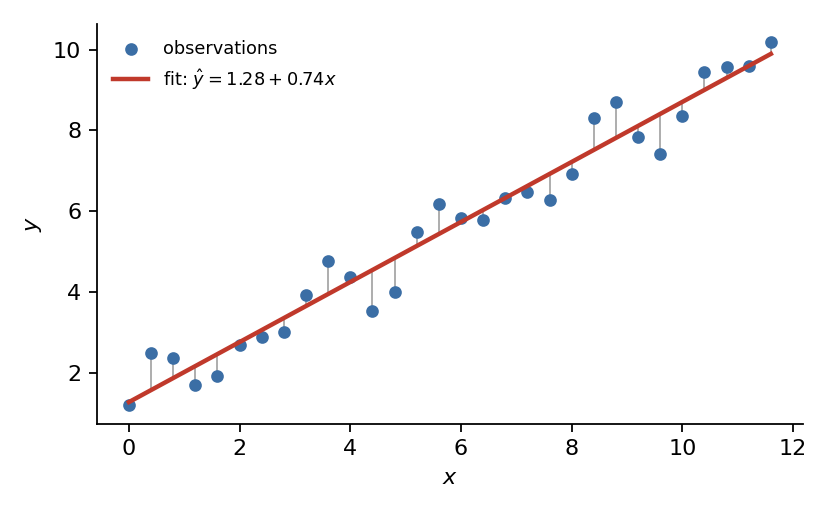
\includegraphics[width=0.7\textwidth]{scatter-fit.png}
\end{center}

\begin{table}[t]
    \centering
    \begin{tabular}{lrrrc}
        \toprule
        Coefficient & Estimate & Std.\ error & $t$ & $p$ \\
        \midrule
        $\hat\beta_0$ (const) & 1.043 & 0.284 & 3.67  & 0.001 \\
        $\hat\beta_1$ ($x$)   & 0.761 & 0.041 & 18.56 & $<$ 0.001 \\
        $\hat\sigma$          & 0.802 &       &       & \\
        $R^2$                 & 0.925 &       &       & \\
        \bottomrule
    \end{tabular}
    \caption{Ordinary least squares, $n = 30$.}
    \label{tbl:estimates}
\end{table}

The residuals look symmetric, which is consistent with, though hardly proof of, the homoskedasticity that Proposition~\ref{prp:gm} assumes:
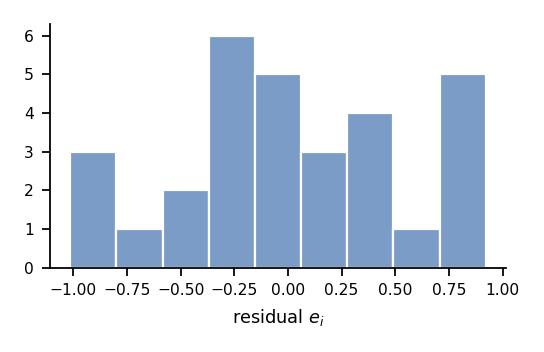
\includegraphics[width=0.45\textwidth]{residuals.png}

\begin{exercise}[Uncentred $R^2$]\label{exr:r2}
Show that if $X$ contains no column of ones, the identity in
\eqref{eq:anova} holds with $\bar y$ replaced by $0$, and that the resulting
\emph{uncentred} $R^2$ lies in $[0,1]$ even though the centred one need not.
\end{exercise}

\begin{solution}
Orthogonality gives $\|y\|^2 = \|\hat y\|^2 + \|e\|^2$ for any $X$, since that statement never mentions $\mathbf{1}$. Dividing by $\|y\|^2$ puts $\|\hat y\|^2 / \|y\|^2$ in $[0,1]$. The centred version subtracts $n \bar y^2$ from both sides, and that subtraction is only legitimate when $\mathbf{1} \in \operatorname{col}(X)$.
\end{solution}

% ----------------------------------------------------------------
\section{Historical note and references}
\label{sec:history}

The method appeared in print first in \cite{legendre1805}, as an appendix on comet orbits, and was published with its probabilistic justification four years later by Gauss \cite{gauss1809}, who claimed to have used it since 1795. The priority dispute is told carefully in \cite[pp.~465--474]{stigler1981}. The projection formulation used here is standard; see \cite[ch.~3]{hansen2022} or \cite[\S1.4]{davidson1993} for textbook treatments, and \cite{strang2016} for the linear algebra. Multiple keys in one command: \cite{legendre1805,gauss1809,stigler1981}.

\begin{thebibliography}{9}
\bibitem{davidson1993} Davidson, R. and MacKinnon, J. G. (1993).
  \emph{Estimation and Inference in Econometrics}. Oxford University Press.
\bibitem{gauss1809} Gauss, C. F. (1809).
  \emph{Theoria Motus Corporum Coelestium}.
\bibitem{hansen2022} Hansen, B. E. (2022).
  \emph{Econometrics}. Princeton University Press.
\bibitem{legendre1805} Legendre, A. M. (1805).
  \emph{Nouvelles m\'ethodes pour la d\'etermination des orbites des com\`etes}.
\bibitem{stigler1981} Stigler, S. M. (1981). Gauss and the invention of least
  squares. \emph{Annals of Statistics}, 9(3), 465--474.
\bibitem{strang2016} Strang, G. (2016).
  \emph{Introduction to Linear Algebra}, 5th ed.
\end{thebibliography}

% ==============================================================
\section{Edge cases}
\label{sec:edge}
% =============================================================

Nothing below is mathematics; it is a checklist. Each subsection states what \emph{should} happen.

\subsection{Inline math}

Adjacent to punctuation: ($x$), [$y$], \{$z$\}, $a$, $b$; $c$: $d$! and $e$?
Two in a row, $u$ $v$, and glued to text, pre$x$post. The paren form
\(a + b\) and \( \tfrac{1}{2} \) with padding.

Escaped currency: \$5 and \$10 million, and a percent sign, 95\%.

A comment containing fake math and a fake environment, all of which must stay inert: % $x^2$ and \begin{theorem} and 
\includegraphics{tiny.png}

Math with braces and backslashes: $\{x : x > 0\}$, $\|v\|_{\infty}$,
$\text{TSS} = \sum_i (y_i - \bar y)^2$, $\overbrace{a+b}^{c}$.

Broken KaTeX (should show an error indicator, not swallow the document):
$\frac{1}{$ and $\undefinedmacro{x}$.

\subsection{Display math, every delimiter}

\[
    \sum_{k=0}^{n} \binom{n}{k} = 2^n
\]

$$
    \int_0^\infty e^{-x^2} \, dx = \frac{\sqrt{\pi}}{2}
$$

\begin{equation}
    \nabla \cdot \mathbf{E} = \frac{\rho}{\varepsilon_0}
\end{equation}

\begin{equation*}
    a^2 + b^2 = c^2
\end{equation*}

\begin{align}
    (x+y)^2 &= x^2 + 2xy + y^2 \\
    (x-y)^2 &= x^2 - 2xy + y^2
\end{align}

\begin{align*}
    e &= My \\
      &= (I - P) y
\end{align*}

\begin{gather}
    \hat y = Py \\
    e = My
\end{gather}

% KNOWN LIMITATION: KaTeX has no `multline` environment, so this block is
% expected to show the KaTeX error styling rather than a rendered formula.
\begin{multline}
    (a + b + c + d + e + f + g + h)^2 = a^2 + b^2 + c^2 + d^2 \\
    + 2(ab + ac + ad + bc + bd + cd) + \dots
\end{multline}

\begin{alignat}{2}
    x &= 1 &\quad y &= 2 \\
    z &= 3 &\quad w &= 4
\end{alignat}

Cases, matrices, and a very wide line that must not create a horizontal scrollbar:

\[
    \mathbb{1}\{i = j\} =
    \begin{cases}
        1 & \text{if } i = j, \\
        0 & \text{otherwise},
    \end{cases}
    \qquad
    P = \begin{pmatrix}
        p_{11} & \cdots & p_{1n} \\
        \vdots & \ddots & \vdots \\
        p_{n1} & \cdots & p_{nn}
    \end{pmatrix}
\]

\begin{equation}
    \hat\beta_{\mathrm{GLS}} = \left( X^\top \Omega^{-1} X \right)^{-1} X^\top \Omega^{-1} y = \left( \sum_{i=1}^{n} \omega_i^{-1} x_i x_i^\top \right)^{-1} \left( \sum_{i=1}^{n} \omega_i^{-1} x_i y_i \right) \quad \text{with} \quad \Omega = \operatorname{diag}(\omega_1, \dots, \omega_n) \quad \text{and} \quad \omega_i > 0 \text{ for all } i
    \label{eq:wide}
\end{equation}

Nested delimiters, for the Tab-out and \verb|\left…\right| pairing:
$\left( a \left( b \right) c \right)$ and $\left[ \frac{a}{b} \right]$.

\subsection{Callout environments}

\begin{theorem}
A theorem with no title argument.
\end{theorem}

\begin{theorem*}
A starred theorem: same box, no number.
\end{theorem*}

\begin{theorem}[A title containing \emph{markup}, math $\sigma^2$ and a colon: like this]
Titles are free text up to the closing bracket.
\end{theorem}

The same title split across two lines is \emph{not} recognised, by design: the
open-fence regex matches a single line, so this stays raw source.

\begin{theorem}[A title that wraps onto
                a second line]
Raw source expected.
\end{theorem}

\begin{lemma}[Contains display math]
\begin{equation}
    \operatorname{tr}(M) = n - k .
    \label{eq:trace}
\end{equation}
And a list:
\begin{itemize}
    \item interior markup keeps rendering,
    \item because the scanner only decorates the fence lines.
\end{itemize}
\end{lemma}

\begin{conjecture}
Recognised, though rarely used.
\end{conjecture}

\begin{note}
The Quarto admonition names work here too: note, tip, warning, important,
caution.
\end{note}

\begin{tip}
A tip box.
\end{tip}

\begin{caution}
A caution box.
\end{caution}

\begin{bogus}
An unrecognised environment is left as raw source, which is what should happen
here.
\end{bogus}

A \verb|\begin{theorem}| that is not alone on its line is also left alone: \begin{theorem} inline.

\subsection{Environments that are not callouts}

\begin{itemize}
    \item An itemize is a list, not a callout.
    \item Nested:
    \begin{enumerate}
        \item first,
        \item second,
        \begin{itemize}
            \item third level.
        \end{itemize}
    \end{enumerate}
    \item An item with math $\varepsilon_i$ and \textbf{bold}.
    \item[custom] An item with a custom label.
\end{itemize}

\begin{enumerate}
    \item one
    \item two
    \item
\end{enumerate}

\begin{description}
    \item[Hat matrix] $P = X(X^\top X)^{-1}X^\top$.
    \item[Residual maker] $M = I - P$.
\end{description}

\subsection{Verbatim and code}

\begin{verbatim}
A verbatim block containing $x^2$, \begin{theorem}, and \item.
KNOWN LIMITATION: the math scanner does not guard verbatim, so the
dollars above are picked up; the list scanner does guard it, so the
\begin{itemize} below stays raw.
\begin{itemize}
    \item not a list
\end{itemize}
\end{verbatim}

\begin{lstlisting}[language=Python]
X = np.column_stack([np.ones(n), x])
beta_hat = np.linalg.solve(X.T @ X, X.T @ y)
\end{lstlisting}

Inline verbatim: \verb|$x^2$| and \texttt{\textbackslash includegraphics}.

\subsection{Sectioning and text styling}

\subsubsection{A third-level heading}

\textbf{Bold}, \emph{emphasis}, \textit{italic}, \texttt{monospace},
\textbf{bold with \emph{nested emphasis}}, and \emph{emphasis spanning
a line break}.

\section*{A starred section}

Starred sectioning should still pick up the heading scale.

\subsection{Images}

Plain, extension omitted (the host resolver tries the common extensions and
honours \verb|\graphicspath|):


\includegraphics{tiny}

With an explicit extension:


\includegraphics{tiny.png}

Half the measure, and the full measure:


\includegraphics[width=0.5\textwidth]{wide-banner.png}


\includegraphics[width=\textwidth]{wide-banner.png}

Other length units and \verb|scale=|, which are ignored (natural size):


\includegraphics[width=3cm]{tiny.png}

\includegraphics[scale=0.5]{tiny.png}

Options in any order, with spaces:

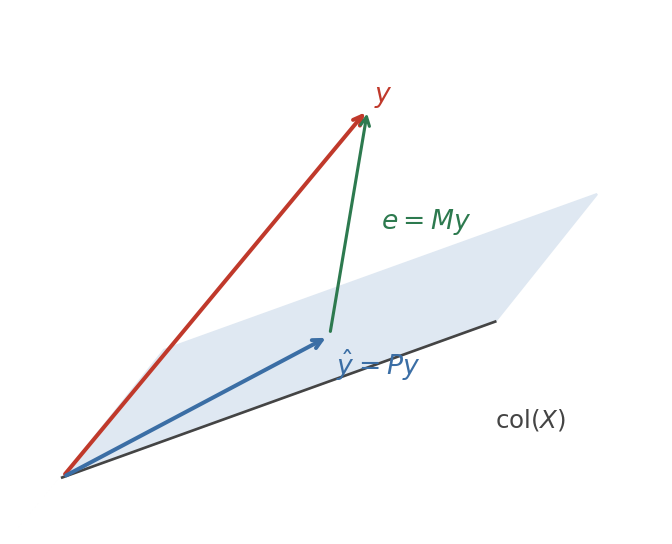
\includegraphics[ keepaspectratio , width = 0.3\linewidth ]{projection.png}

An extreme aspect ratio:


\includegraphics[width=0.2\textwidth]{tall-column.png}

A path with a space, and an uppercase extension:

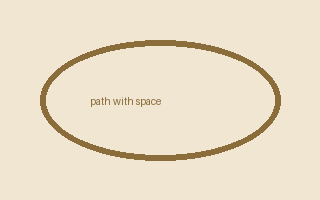
\includegraphics{plot with space.png}


\includegraphics{upper-case.PNG}

A missing file (placeholder, not a broken layout):

\includegraphics{no-such-file.png}

Two on one line: 
\includegraphics{tiny.png} 
\includegraphics{tiny.png}

Inside a figure, with a caption and label:

\begin{figure}[h]
    \centering
    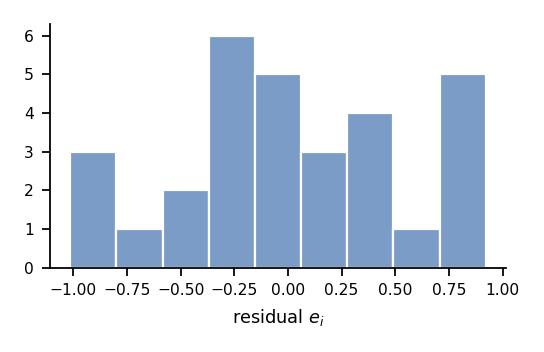
\includegraphics[width=0.6\textwidth]{residuals.png}
    \caption{Residual histogram.}
    \label{fig:residuals}
\end{figure}

A command split across lines stays raw source by design (a replace decoration may not span a line break):

\includegraphics[width=0.5\textwidth]{%
    tiny.png}

\subsection{Cross-references and citations}

Chalk resolves \verb|@key| references in Markdown only; in \LaTeX{} the
commands stay raw source, which is correct because the numbers come from the
compiler. Check that they are at least highlighted sanely:
Theorem~\ref{thm:projection}, equation~\eqref{eq:normal}, page~\pageref{sec:setup},
\autoref{lem:idem}, \cite[p.~12]{hansen2022}, \nameref{sec:example}.

An \verb|@|-sign in prose, contact@example.com, and in math, $a @ b$, must not
be touched either.

\subsection{Long lines}

A single very long paragraph line, no hard wraps, to check soft wrapping and hanging indent: the ordinary least squares estimator solves the normal equations, and because the residual maker $M$ annihilates the column space of $X$, every projection identity in this document, including the analysis-of-variance decomposition and the Gauss--Markov comparison of variance matrices, reduces to the single statement that $y$ splits orthogonally into a fitted part and a residual part.

\subsection{Unterminated blocks (kept last on purpose)}

An unclosed environment, which must stay raw source rather than swallowing the
rest of the file:

\begin{theorem}
This theorem is never closed.

An unclosed display at the end of the document:

\[
    \lim_{n \to \infty} \hat\beta_n = \beta

\end{document}
